% Intended LaTeX compiler: pdflatex


\documentclass[12pt]{article}
% \usepackage[includeheadfoot,margin=1.0in,hmargin=1.0in,vmargin=0.5in]{geometry} % for normal margins
\usepackage[includeheadfoot,margin=1.5in,hmargin=1.5in,vmargin=0.5in]{geometry} % for insanely wide margins
% \usepackage[includeheadfoot,margin=2.0in,hmargin=2.0in,vmargin=0.5in]{geometry} % for insanely wide margins
\usepackage{float}


\usepackage{algorithm}
\usepackage{amsmath}
\usepackage{ifxetex}
\ifxetex
  \usepackage{fontspec,xltxtra,xunicode}
  \defaultfontfeatures{Mapping=tex-text,Scale=MatchLowercase}
  \setromanfont{Garamond Premier Pro}
%  \setromanfont{Adobe Caslon Pro}
 \setsansfont{Gotham Narrow Bold}
  \setmonofont{Myriad Pro}
\else
  \usepackage[mathletters]{ucs}
  \usepackage[utf8x]{inputenc}
\fi
\usepackage{url}
\usepackage{paralist}
\usepackage{graphicx}
\usepackage{tikz}
\usepackage{calc}
\usepackage{eso-pic}
\usepackage{etoolbox}
\usepackage{xcolor}
\PassOptionsToPackage{hyperref,x11names}{xcolor}
\definecolor{pinterestred}{HTML}{C92228}
\definecolor{ulyssesbutterflyblue}{HTML}{1464F4}
\definecolor{signalflare}{HTML}{FB782C}
\definecolor{niceorange}{HTML}{77CC6D}
\definecolor{highlighteryellow}{HTML}{FFFF01}
\definecolor{ghostlygrey}{HTML}{000000}
\definecolor{firstcolor}{HTML}{00ADEF}
\definecolor{secondcolor}{HTML}{DD3E74}
\definecolor{periodblue}{HTML}{12239e}
\definecolor{denimblue}{HTML}{3A5F90}
\definecolor{electricblue}{HTML}{05ADF3}


\newtoks\leftheader 
\newtoks\leftheaderurl
\newtoks\coverimage


\hyphenpenalty=5000 
\tolerance=1000

%This macro is to make cleaner the specification of the titling font
\newfontfamily\mytitlefont[Color={highlighteryellow}]{Gotham Narrow Bold}
\newfontfamily\myauthorfont[Color={highlighteryellow}]{Gotham Narrow Bold}
\newfontfamily\mybluefont[Color=electricblue]{Gotham Narrow Bold}
\DeclareTextFontCommand{\textbf}{\bfseries\color{electricblue}}
\DeclareTextFontCommand{\textit}{\itshape}


\usepackage{textcase}

\pagenumbering{arabic}
\makeatletter

%This macro now controls the position of the background pic
%Please do not change from here
\newcommand\BackgroundPic{%
\put(0,0){%
\parbox[b][\paperheight]{\paperwidth}{%
\vfill
\centering
%inside the tikzpicture environment, you can do anything you want with the image
\begin{tikzpicture}

\node [inner sep=0pt,outer sep=0pt] at (0,0) {\includegraphics[width=\paperwidth,height=\paperheight]{\the\coverimage}};

\node at  (0,5) [opacity=1.0] {\parbox[b][0.5\textheight]{\textwidth}{%
  \begin{raggedright}
  \leavevmode
    \vskip 1cm
  {\mytitlefont\fontsize{75}{85}\bfseries{\@title}\par}
    \vskip 1cm
    
    %{\myauthorfont\fontsize{30}{40}{{\bfseries{\@degree}\par}}}

\vfill
\end{raggedright}}};
\node at (0,-8) [opacity=1] {\parbox[b][0.3\textheight]{\textwidth}{%
\begin{raggedright}
\vfill
{\myauthorfont\Large {\@author}}
    \newline
          {\myauthorfont\Large \href{mailto:jay@storytelling.nyc}{jay@storytelling.nyc}}
        \newline
{\myauthorfont\Large
\href{http://storytelling.nyc}{Storytelling.NYC}}
\newline
{\myauthorfont\Large © 2017 \@author}
    \newline
%{\myauthorfont\Large Private and Confidential}
 %   \newline
        \newline
    {\myauthorfont\Large \@date\par}
%{\myauthorfont\Large \href{http://jaydixit.com}{\@degree }}
\end{raggedright}
}};
\end{tikzpicture}
%Don't change
\vfill
}}}
%This macro executes a hook at the beginning of the document that  puts the background correctly. 
\AtBeginDocument{\AddToShipoutPicture*{\BackgroundPic}}
\AtBeginDocument{\globalcolor{ghostlygrey}}



%The maketitle macro now only includes the titling and not the background. 
\def\maketitle{ \newgeometry{margin=1in} \thispagestyle{empty} \vfill \null \cleardoublepage\restoregeometry}



\setcounter{secnumdepth}{0}




\usepackage{fancyhdr}
\pagestyle{fancy}
\renewcommand{\sectionmark}[1]{\markboth{#1}{}}
\lhead{\href{\the\leftheaderurl}{\the\leftheader}}
\chead{}
\rhead{\@title: {\nouppercase{\leftmark}}}
\lfoot{}
\cfoot{}
\rfoot{}
\usepackage{listings}
\setlength{\parindent}{0pt}
\setlength{\parskip}{12pt plus 2pt minus 1pt} %Space between paragraphs
\usepackage{fancyvrb}
\usepackage{enumerate}
\usepackage{ctable}
\setlength{\paperwidth}{8.5in}
\setlength{\paperheight}{11in}
  \tolerance=1000
\usepackage{tocloft}
\renewcommand{\cftsecleader}{\cftdotfill{\cftdotsep}}
\usepackage[normalem]{ulem}


\makeatletter
\newcommand{\globalcolor}[1]{%
  \color{#1}\global\let\default@color\current@color
}
\makeatother

\newcommand{\textsubscr}[1]{\ensuremath{_{\scriptsize\textrm{#1}}}}

\usepackage{enumitem}
\newlist{mylist}{enumerate}{10} 
%\setlist{nolistsep}
\setlist{topsep=0pt}
\renewcommand{\labelitemi}{\raise 0.25ex\hbox{\tiny$\bullet$}}
\renewcommand{\labelitemii}{\raise 0.25ex\hbox{\tiny$\bullet$}}
\renewcommand{\labelitemiii}{\raise 0.25ex\hbox{\tiny$\bullet$}}
\renewcommand{\labelitemiv}{\raise 0.25ex\hbox{\tiny$\bullet$}}
\renewcommand{\labelitemv}{\raise 0.25ex\hbox{\tiny$\bullet$}}
\renewcommand{\labelitemvi}{\raise 0.25ex\hbox{\tiny$\bullet$}}
\renewcommand{\labelitemvii}{\raise 0.25ex\hbox{\tiny$\bullet$}}
\renewcommand{\labelitemviii}{\raise 0.25ex\hbox{\tiny$\bullet$}}
\renewcommand{\labelitemix}{\raise 0.25ex\hbox{\tiny$\bullet$}}
\renewcommand{\labelitemx}{\raise 0.25ex\hbox{\tiny$\bullet$}}

\setlistdepth{10}
\setlist[itemize,1]{label=\raise 0.25ex\hbox\tiny$\bullet$}
\setlist[itemize,2]{label=\raise 0.25ex\hbox\tiny$\bullet$}
\setlist[itemize,3]{label=\raise 0.25ex\hbox\tiny$\bullet$}
\setlist[itemize,4]{label=\raise 0.25ex\hbox\tiny$\bullet$}
\setlist[itemize,5]{label=\raise 0.25ex\hbox\tiny$\bullet$}
\setlist[itemize,6]{label=\raise 0.25ex\hbox\tiny$\bullet$}
\setlist[itemize,7]{label=\raise 0.25ex\hbox\tiny$\bullet$}
\setlist[itemize,8]{label=\raise 0.25ex\hbox\tiny$\bullet$}
\setlist[itemize,9]{label=\raise 0.25ex\hbox\tiny$\bullet$}
\setlist[itemize,10]{label=\raise 0.25ex\hbox\tiny$\bullet$}
\renewlist{itemize}{itemize}{10}





\definecolor{azure}{HTML}{f2feff}

\usepackage{lipsum}
\usepackage{tikz}
\usetikzlibrary{backgrounds}
\makeatletter

\tikzset{%
  fancy quotes/.style={
    text width=\fq@width pt,
    align=justify,
    inner sep=1em,
    anchor=north west,
    minimum width=\linewidth,
  },
  fancy quotes width/.initial={.8\linewidth},
  fancy quotes marks/.style={
    scale=8,
    text=black,
    inner sep=0pt,
  },
  fancy quotes opening/.style={
    fancy quotes marks,
  },
  fancy quotes closing/.style={
    fancy quotes marks,
  },
  fancy quotes background/.style={
    show background rectangle,
    inner frame xsep=0pt,
    background rectangle/.style={
      fill=azure,
      rounded corners,
    },
  }
}

\newenvironment{fancyquotes}[1][]{%
\noindent
\tikzpicture[fancy quotes background]
\node[fancy quotes opening,anchor=north west] (fq@ul) at (0,0) {``};
\tikz@scan@one@point\pgfutil@firstofone(fq@ul.east)
\pgfmathsetmacro{\fq@width}{\linewidth - 2*\pgf@x}
\node[fancy quotes,#1] (fq@txt) at (fq@ul.north west) \bgroup}
{\egroup;
\node[overlay,fancy quotes closing,anchor=east] at (fq@txt.south east) {''};
\endtikzpicture}
\makeatother


\usepackage{setspace}
\usepackage{lipsum}
\usepackage{etoolbox}
\AtBeginEnvironment{quote}{\singlespace\vspace{-\topsep}\small}
\AtEndEnvironment{quote}{\vspace{-\topsep}\endsinglespace}


\usepackage[sc]{titlesec}
\titlespacing*{\section}{0pt}{6pt}{7pt}
\titlespacing*{\subsection}{0pt}{0pt}{7pt}
\titlespacing*{\subsubsection}{0pt}{6pt}{5pt}

\titleformat*{\section}{\normalfont\fontsize{36}{36}\raggedright\bfseries\sffamily\color{pinterestred}}
\titleformat*{\subsection}{\normalfont\fontsize{20}{20}\scshape\color{electricblue}}
\titleformat*{\subsubsection}{\normalfont\fontsize{12}{8}\raggedright\bfseries\rmfamily\color{pinterestred}}
\titleformat*{\paragraph}{\normalfont\normalsize\raggedright\bfseries\rmfamily\color{electricblue}}
\titleformat*{\subparagraph}{\normalfont\fontsize{14}{14}\raggedright\bfseries\ttfamily\color{pinterestred}}
\usepackage[breaklinks=true,linktocpage,xetex]{hyperref} 
\hypersetup{colorlinks, citecolor=electricblue,filecolor=electricblue,linkcolor=electricblue,urlcolor=electricblue}




      

\setcounter{secnumdepth}{0}
\setcounter{tocdepth}{3}
\leftheader{Storytelling.NYC}
\leftheaderurl{http://storytelling.nyc}
\coverimage{/Users/jay/emacs/emacs-settings/new-latex-templates/images/image1.jpg}
\author{Jay Dixit}
\date{\today}
\title{}
\hypersetup{
 pdfauthor={Jay Dixit},
 pdftitle={},
 pdfkeywords={},
 pdfsubject={},
 pdfcreator={Emacs 25.1.1 (Org mode 9.1.3)}, 
 pdflang={English}}
\begin{document}

\tableofcontents
\newpage
\section{The Art of Storytelling}
\label{sec:org3c0fedb}
Training Intensive \\
Prepared Exclusively for Frank Løfqvist
Monday November 27, 2017.

\textbf{Jay Dixit} \\
\href{http://www.storytelling.nyc}{www.storytelling.nyc} \\
\href{mailto:jay@storytelling.nyc}{jay@storytelling.nyc} \\

\begin{center}

\includegraphics[width=.9\linewidth]{/Users/jay/Dropbox/github/org-html-webslides/assets/img/storytelling-nyc-logo-new-face.png}
\end{center}

\section{Intro}
\label{sec:orgee2c868}

\subsection{The Neuroscience of Storytelling}
\label{sec:orge35c3b0}
Why is storytelling so effective at changing people's attitudes and behavior?


\subsection{The Neuroscience of Storytelling}
\label{sec:org9a5d508}
Because stories affect the brain in a way facts and figures can't---a phenomenon known as ``Narrative Transportation.''

\subsection{Narrative Transportation}
\label{sec:orge239ae4}

Narrative transportation is the total absorption we feel when we're fully immersed in a story. It's that wonderful feeling of racing to the end of a great mystery novel, getting lost in the world of a movie, or listening rapt to a spellbinding story.

\subsection{Storytelling bypasses the evaluative brain}
\label{sec:org7dbbcec}

It's natural to want to prove to your customer that your product is great and explain all the reasons why it's better than other products. That's why most of us try to persuade customers using logic: Facts and figures, statistics, reasons, and quotes from expert authorities.

\subsection{Storytelling vs. Information}
\label{sec:orga8c85b5}

But research shows that merely presenting information activates the evaluative regions of the brain---the rational, critical parts that make consumers skeptical and defensive when they sense you're trying to sell them something. Information you present is evaluated critically, and the mind is resistant to persuasion, asking:
\begin{itemize}
\item Do I agree with this?
\item Is this true?
\item Can I spot any flaws with this?
\end{itemize}

\subsection{Storytelling is different.}
\label{sec:org029952e}
By inducing narrative transportation, stories bypass the evaluative region of the brain, activating the experiential and emotional regions instead. The listener is placed in a receptive state of mind in which counterarguing is reduced. Instead of looking for flaws in the argument, your listener is transported into the world of the story. In this state, stories ignite their imagination, move their emotions, and prime them to be persuaded and take action.

\subsection{Neurological Effects of Storytelling}
\label{sec:orga1c5100}

\begin{center}
\includegraphics[width=.9\linewidth]{/Users/jay/Downloads/Screenshots/narrative-transport.png}
\end{center}


\subsection{Stories captivate attention}
\label{sec:orgf5a5a0e}
\begin{quote}
``The audience will not tune in to watch information. You wouldn't, I wouldn't. No one would or will. The audience will only tune in and stay tuned to watch DRAMA.''
---David Mamet
\end{quote}

\subsection{Stories captivate attention}
\label{sec:org25884b4}
This quote is about what makes for captivating television, but the principle applies equally to sales. When you tell a story, people perk up, lean forward, and start listening, whether they want to or not. According to research by neuroeconomist Paul Zak, hearing a suspenseful story literally changes the brain, triggering the release of the stress hormone cortisol, which amplifies attention and focus. In other words, stories can't help but make us sit up and pay attention.

\subsection{Stories Simulate Reality}
\label{sec:org4b3acc4}
The sensory regions of the brain don't distinguish between stories and real experiences. When we hear stories, the brain regions that process the sights, sounds, tastes, and movement of real life are activated. Stories about food activate our sensory cortex, stories about movement activate the motor cortex.

In other words, if I tell you a story about walking through a pine forest and smelling the sharp scent of woodsmoke, the olfactory sensory regions of your brain activate exactly as they would if you were actually trudging through the snow with me and smelling the fire yourself. That's far more engaging than hearing facts, figures, and arguments. Since narrative simulates reality in the brain, you're more engaged, you enjoy the experience more, you understand it better, and you remember it longer.

\subsection{Stories Create Meaning}
\label{sec:org1af359e}

Our senses pull in trillions of pieces of data every second, way too much for our conscious minds to process. To find order in all the chaos, our brains are wired to look for patterns. And there's one kind of pattern the brain loves above all else: cause and effect.

When our caveman and cavewoman ancestors drank from a muddy puddle and immediately got sick, it was that pattern-seeking mechanism that enabled them to realize that the two events were connected---that the water was contaminated and had caused the illness.

That's why stories affect us so powerfully---because they explain cause and effect. Neuroscientist Antonio Damasio puts it this way: ``The problem of how to make all this wisdom understandable, transmissible, persuasive, enforceable---in a word, of how to make it stick---was faced and a solution found. Storytelling was the solution.''

\subsection{Emotion}
\label{sec:org2642544}

In research on the neuroscience of decision-making, Antonio Damasio showed that when people get brain damage in the emotional centers of the brain, they're unable to make decisions. Without emotions, these brain-damaged patients are literally unable to form the impulse to take action. Instead they spend hours talking through the pros and cons of picking up a blue pen vs. picking up a black pen.

In other words: Emotions are the only thing that can move people to take action. If you want people to work for you, buy your product, or invest in your company, you need to engage their emotions.

How do you reach people on an emotional level? Through storytelling. Neuroimaging studies show that when evaluating brands, consumers make assessments using emotions and experiences, not attributes, features, or facts. Other research shows that customers' emotional responses to ads are what determine their intent to purchase.

It's simple: If you want someone to act, you need to arouse their emotions and make them feel something. And the best way to do that is through story.

\subsection{Storytelling is the most powerful mode}
\label{sec:org8362357}

Storytelling is more effective than merely offering up information. But creating your story and knowing how to tell it might seem like problems too tough to solve. That's where Storytelling.NYC comes in. We synthesize the science and empower you with the techniques to capture an audience's attention, enchant them with your story, and inspire them to action. Don't wait another minute. Gain a step on your competition by becoming a master storyteller today!

\subsection{Curiosity}
\label{sec:org5630c3b}
\begin{center}

\includegraphics[width=.9\linewidth]{/Users/jay/Dropbox/github/org-html-webslides/assets/img/curiosity-icon.jpg}
\end{center}

\section{Curiosity}
\label{sec:org611b907}
\begin{center}

\includegraphics[width=.9\linewidth]{/Users/jay/Dropbox/github/org-html-webslides/assets/img/videogame-brain-desire.png}
\end{center}

\section{Don't let the \textbf{rope} go \textbf{slack}}
\label{sec:org64c2e01}
\begin{center}
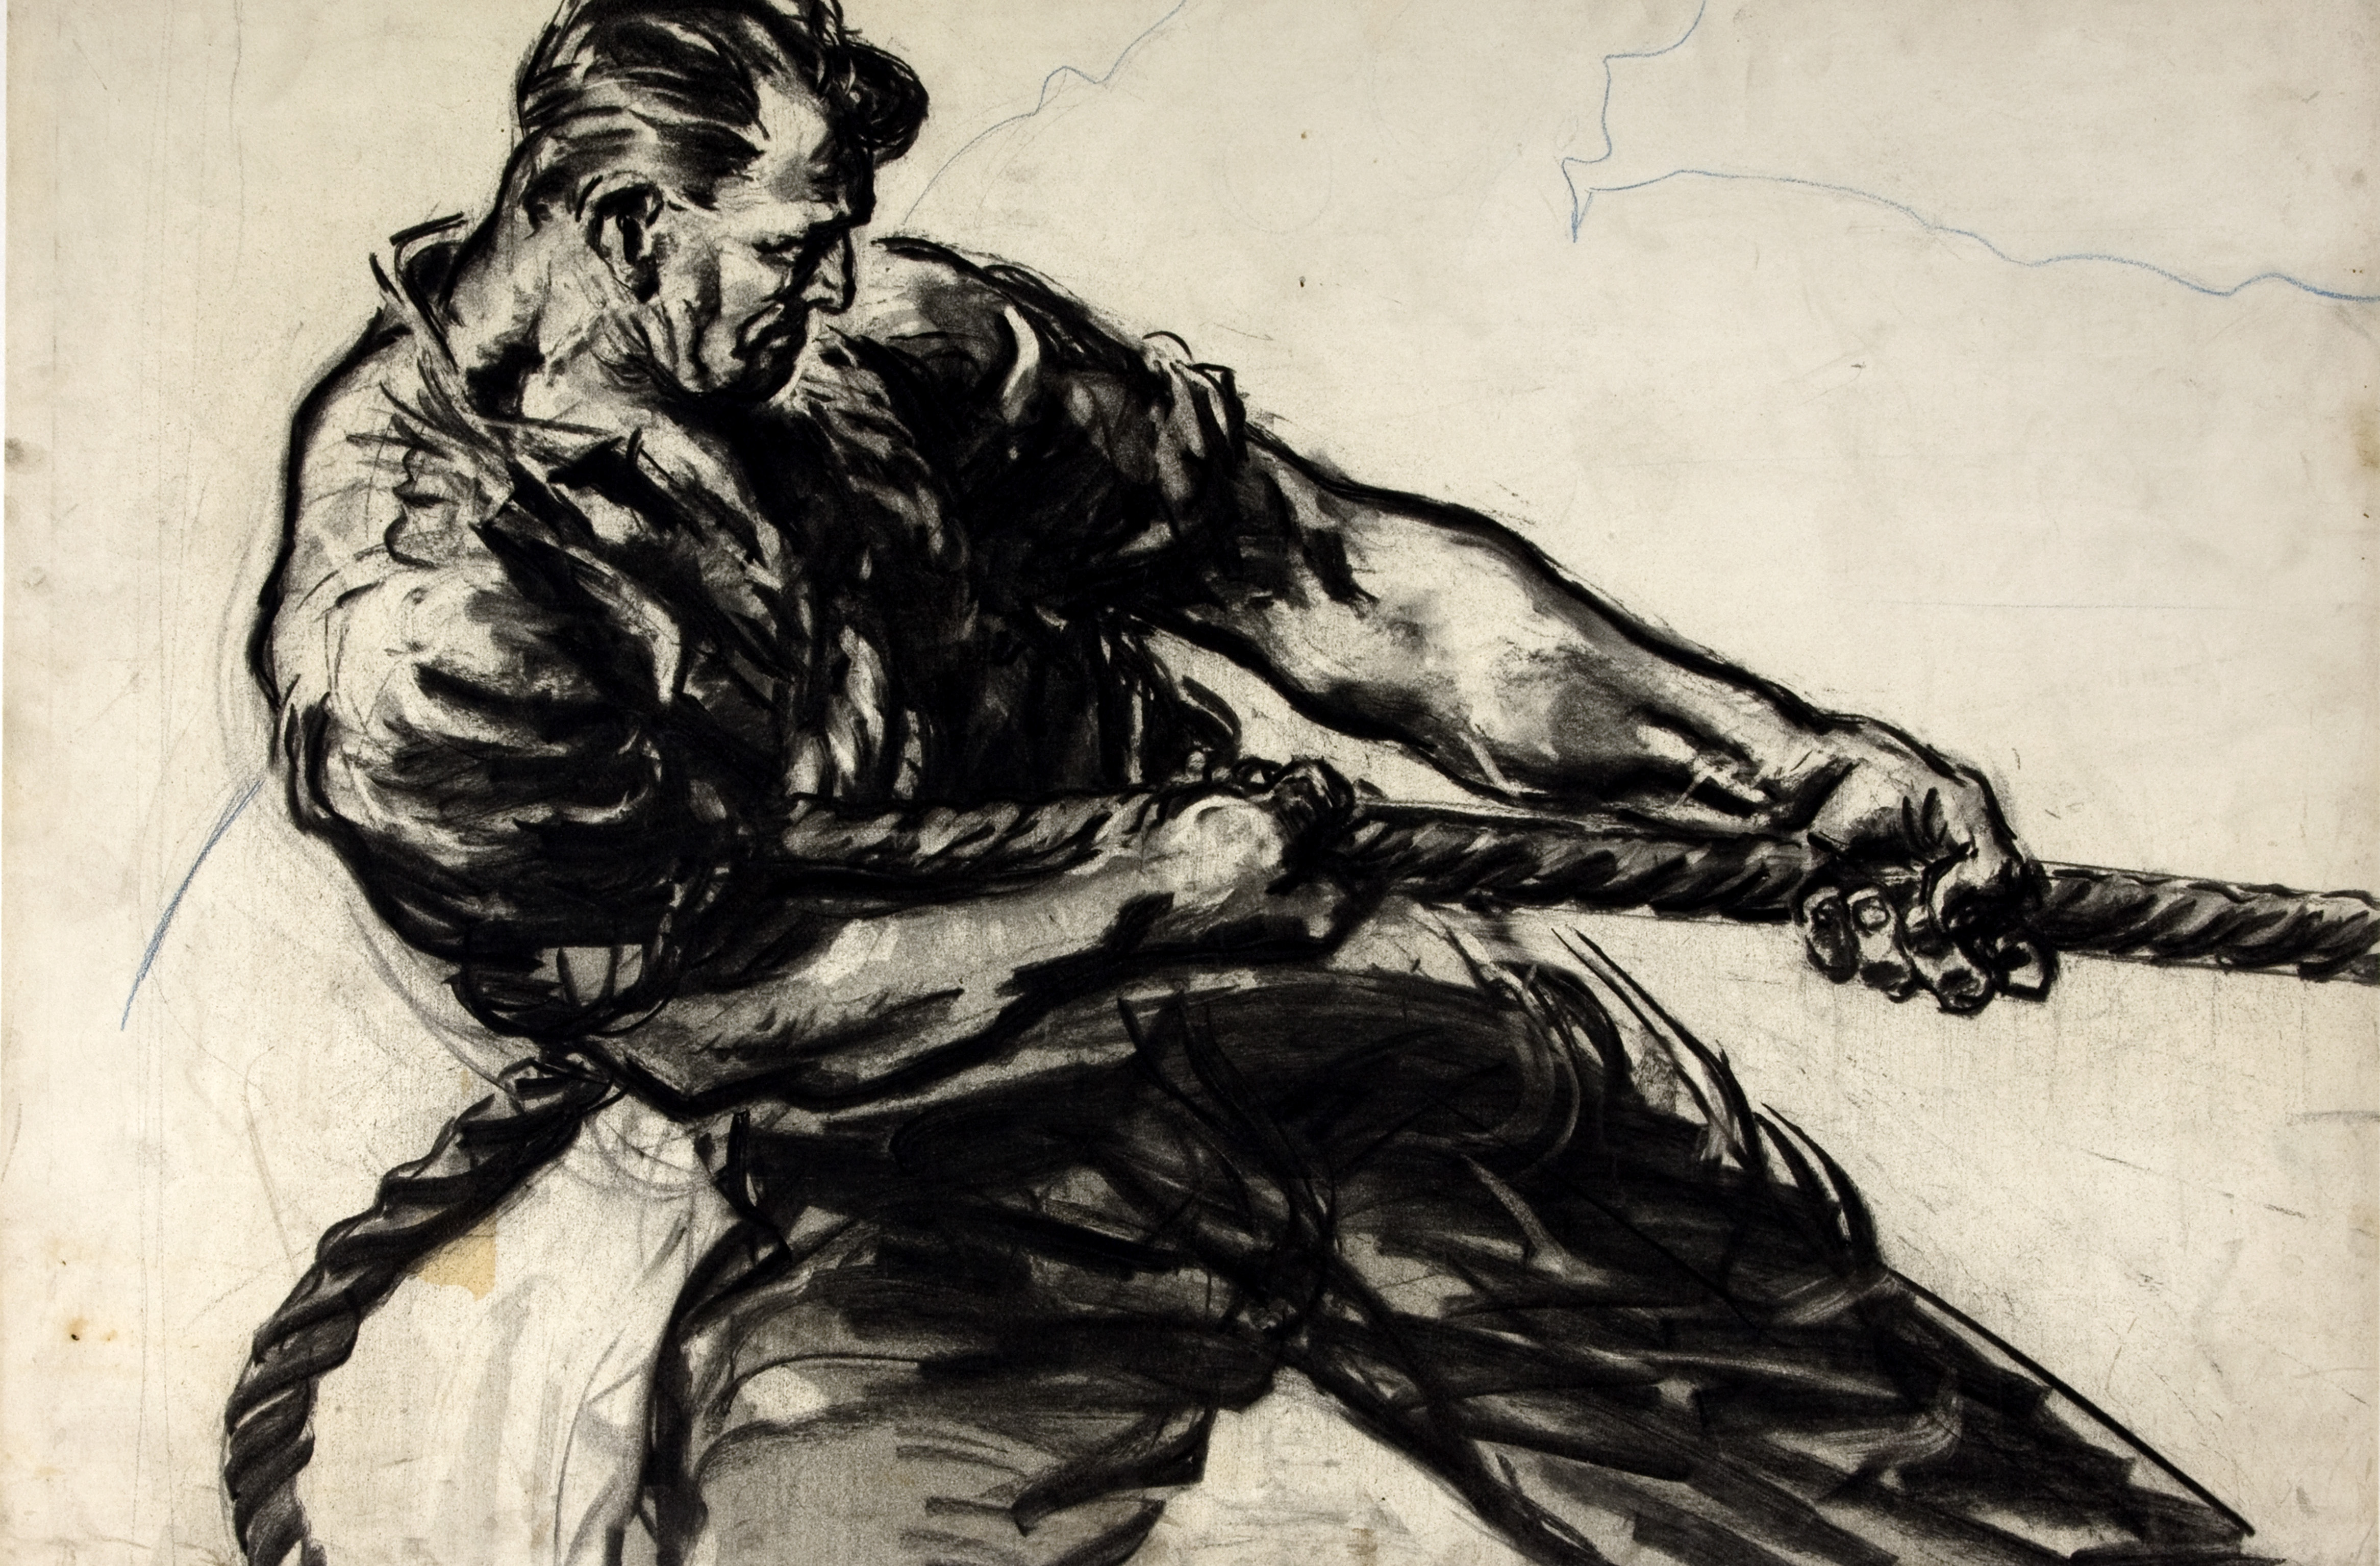
\includegraphics[width=.9\linewidth]{/Users/jay/Dropbox/github/org-html-webslides/assets/img/man_heaving_on_rope.png}
\end{center}

\section{Curiosity}
\label{sec:orge85d8cc}
\begin{center}

\includegraphics[width=.9\linewidth]{/Users/jay/Dropbox/github/org-html-webslides/assets/img/curiosity-icon.jpg}
\end{center}

\section{The Elements of Storytelling}
\label{sec:orgb9a170c}
\begin{center}
\includegraphics[width=.9\linewidth]{/Users/jay/Pictures/2017/2017-11-27-export_2.jpg}
\end{center}

\section{The \textbf{Elements} of \textbf{Storytelling}}
\label{sec:org626e29f}
\begin{enumerate}
\item Goal
\item Obstacle
\item Stakes
\item Strategies
\item Outcome
\end{enumerate}


\section{1. Desire / Goal}
\label{sec:org332842d}
\begin{quote}
"When I used to teach creative writing, I would tell the students to make their characters want something right away---even if it's only a glass of water.

Characters paralyzed by the meaninglessness of modern life still have to drink water from time to time. One of my students wrote a story about a nun who got a piece of dental floss stuck between her lower left molars, and who couldn't get it out all day long. I thought that was wonderful. The story dealt with issues a lot more important than dental floss, but what kept readers going was anxiety about when the dental floss would finally be removed.

Nobody could read that story without fishing around in his mouth with a finger."
---Kurt Vonnegut
\end{quote}

\section{1. Desire (Goal)}
\label{sec:orga72f36c}


\section{2. Obstacle}
\label{sec:org785a041}

\section{3. Stakes}
\label{sec:org5c7e4a7}

\section{The writer \textbf{must} answer these \textbf{three questions}.}
\label{sec:org04c6a34}
\begin{enumerate}
\item \textbf{What} is going to happen? (suspense) / \textbf{What} happens? (outcome)
\item \textbf{How} does the character pursue their goal or escape their dilemma? (strategies)
\item \textbf{Why} is the character taking the action they're taking? (desire)
\end{enumerate}

\section{\textbf{How} will the character achieve their goal or escape their dilemma?}
\label{sec:orgeff6923}
This is also known as\ldots{} \textbf{strategies}.


\section{4. Strategies - \textbf{How} will the character achieve their goal or escape their dilemma?}
\label{sec:org5b687d5}

\begin{center}
\includegraphics[width=.9\linewidth]{/Users/jay/Dropbox/storytelling-assets/Bourne-Identity-006.jpg}
\end{center}


\section{5. Outcome}
\label{sec:orgd9572a9}


\section{Louis CK and his dog}
\label{sec:org8555bd2}
\url{https://www.youtube.com/watch?v=VMeXGE\_a8Gg}


\section{2. Action / Reaction}
\label{sec:org1fa8163}
\begin{center}
\includegraphics[width=.9\linewidth]{/Users/jay/Dropbox/storytelling-assets/Facial_Expression_Study_by_signedup.jpg}
\end{center}

\section{2. Action / Reaction}
\label{sec:org032d430}
Not just the action\ldots{}

\begin{center}
\includegraphics[width=.9\linewidth]{/Users/jay/Dropbox/storytelling-assets/suspense-storytelling-images/action--car-crash.png}
\end{center}

\section{2. Action / Reaction}
\label{sec:org7da8b15}
\ldots{}but also its effect on the character.

\begin{center}
\includegraphics[width=.9\linewidth]{/Users/jay/Dropbox/storytelling-assets/suspense-storytelling-images/reaction--car-crash.png}
\end{center}

\section{Cause and effect}
\label{sec:orgd7880e4}
What's the difference between a list and a story?

\section{So, \textbf{how} do we \textbf{show} cause and effect in a story?}
\label{sec:org68907f6}
Two ways:

\begin{enumerate}
\item Desire/Goal (explain the \textbf{why})
\item Action / Reaction
\end{enumerate}


\section{A list}
\label{sec:org80da360}

\begin{quote}
Queen dies, king dies.
\end{quote}

\section{A story}
\label{sec:orgf737ebb}

\begin{quote}
Queen dies, king dies of grief.
\end{quote}



\section{The Elements of Storytelling}
\label{sec:orgfed786b}
\begin{center}
\includegraphics[width=.9\linewidth]{/Users/jay/Pictures/2017/2017-11-27-export_2-2.jpg}
\end{center}

\section{Cause and Effect}
\label{sec:org86c3a97}
Louis CK's car chase: \\
\url{https://www.youtube.com/watch?v=679wktf2nOE}

\section{``My product is the solution to the problem''}
\label{sec:org6b69237}
Google ad: Reunion

\section{How to inspire employees?}
\label{sec:org38c9253}

When employees are facing obstacles and missing deadlines, how to give them hope and belief in the program and make them feel inspired and motivated?

Perhaps by telling one of two stories:

\subsection{1. Typical customer (who we're helping) as protagonist}
\label{sec:org35f9dc4}
``\href{https://www.youtube.com/watch?v=u4ZoJKF\_VuA}{People don't buy what you do. They buy why you do it}.''

\begin{itemize}
\item our mission / vision
\item why do we offer banking services?
\item because we believe in people. And we want to help achieve their full potential
\begin{itemize}
\item Story: ``Meet Janice. Janice wanted to buy a home for her and her daughter but she couldn't afford\ldots{} we helped her achieve her dream.''
\item could be a composite character, or could be a real employee
\end{itemize}
\end{itemize}

\subsection{2. Employee as protagonist, modeling the behavior we want to inspire in employees}
\label{sec:orgfbe5a73}
At this bank, we see obstacles not as challenges but as opportunities to grow and learn to be more than we are

If the behavior we want to instill is rising to the occasion and using ingenuity to solve problems, then it could be a story along these lines:

``Meet James. James was the VP of this department. He encountered an impossible problem. Instead of getting discouraged, he asked himself: how can I be resourceful? By doing this, he succeeded\ldots{}''


\section{The End}
\label{sec:org6b810fd}
\end{document}
